
\section{Site algemeen}\label{sitealgemeen}
In dit hoofdstuk worden de overige functionaliteiten van de website uitgelegd.

\subsection{Responsive Design}\label{responsivedesign}

\drupalpath is op gezet met een Responsive Design. Dit houdt in dat de website zijn uiterlijk aanpast naar de resolutie van verschillende platformen (bijvoorbeeld een mobile telefoon of tablet). 

Andere platformen hebben vaak kleinere browser vensters. Het design van Dimpact zal hier rekening mee houden zodat de website functioneel en overzichtelijk blijft. Dit kun je ook in je eigen browser testen door de breedte van de browser handmatig te veranderen.
\subsection{Favorieten}\label{favorieten}

Via de \usemodule{views} en \usemodule{flag} module wordt het voor medewerkers mogelijk om pagina's als "favoriet" aan te merken. De lijst van favorieten is vervolgens terug te vinden op het dashboard\seeone{dashboard}. Er wordt een nieuw flag type aangemaakt met de volgende settings:
\begin{itemize}
\item Title: "Favoriet" (machine name: "favorite")
\item Flag link text: "Toevoegen als favoriet"
\item Unflag link text: "Verwijderen uit favorieten"
\item Flag access: medewerker- en redacteurrollen
\item Bundles: agenda, basic page, blog, wiki
\item Display link as field: aanvinken
\end{itemize}
Voor alle overige settings wordt de standaardinstelling gebruikt. Met de laatste setting wordt een link toegevoegd aan de detailpagina's die in de favorieten kunnen worden gezet.



\subsection{Taxonomie}\label{taxonomie}

Taxonomie wordt gebruikt voor lijsten van woorden. Bijvoorbeeld: de lijst �FAQ categorie�n� bevat de woorden 'Netwerk' en 'Werkplekken'. Taxonomie lijsten kunnen altijd aangepast worden.

\bigskip

\begin{center}
	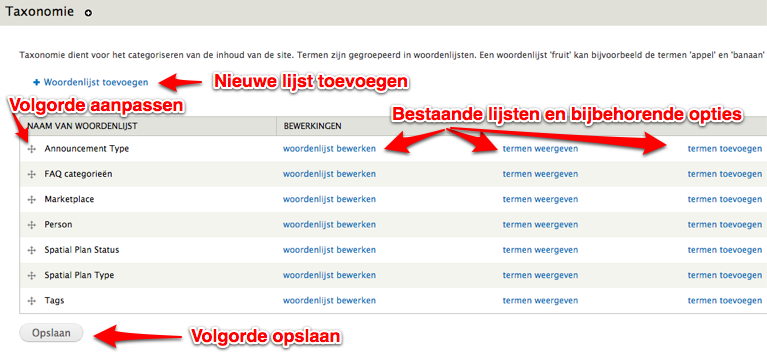
\includegraphics[width=\textwidth]{img/taxonomie2.png}
\end{center}

\subsubsection{Woorden aan woordenlijsten toevoegen}

Ga naar het overzicht van alle woordenlijsten. Klik op 'Termen toevoegen' bij de lijst waaraan je woorden wil toevoegen. Vul bij het veld 'Naam' het woord in en vul eventueel een beschrijving in. Klik onderaan de pagina op de knop 'Opslaan' om het woord aan de lijst toe te voegen. Herhaal deze stappen om meerdere woorden toe te voegen aan de woordenlijst. 

\subsubsection{Woorden in woordenlijsten bewerken}

Het is mogelijk om specifieke woorden uit lijsten te bewerken. Klik op 'Termen weergeven' bij de betreffende lijst.
Klik op 'Bewerken' bij het betreffende woord, vervolgens kun je de wijzigingen doorvoeren. Klik op de knop 'Opslaan' om de wijzigingen op te slaan.

\subsubsection{Woorden uit woordenlijsten verwijderen}

Het is mogelijk om specifieke woorden uit lijsten te verwijderen. Klik op 'Termen weergeven' bij de betreffende lijst.
Klik op 'Bewerken' bij het betreffende woord, om het woord te verwijderen klik je onderaan de op de knop 'Verwijderen'. Na het bevestigen zal het woord definitief en onherstelbaar verwijderd worden.


\subsection{Zoeken}\label{zoeken}

Voor \drupalpath wordt de \emph{Solr module} gebruikt, deze module vervangt de standaard \emph{Drupal Search module}. 
De \emph{Solr module} biedt naast de standaard zoek functionaliteit ook meer geavanceerde functionaliteiten zoals zoeken in bijlagen, markeren van zoekwoorden en de mogelijkheid tot het aanpassen van de \emph{Bias settings}. 

\subsubsection{Bias settings}

\emph{Bias settings} maken het mogelijk inhoud voorrang te geven in de zoekresultaten. Je kunt bijvoorbeeld het inhoudstype \emph{Nieuws} meer punten geven dan het inhoudstype \emph{Bekendmaking}. Hoe hoger het aantal toegekende punten hoe meer voorrang het krijgt. 

Ga naar \drupalpath{admin/config/search/apachesolr} en klik vervolgens op \emph{Bias} bij de betreffende website om de \emph{Bias settings} aan te passen. Let op: het is niet aangeraden om zonder voldoende kennis deze settings aan te passen.

\begin{center}
	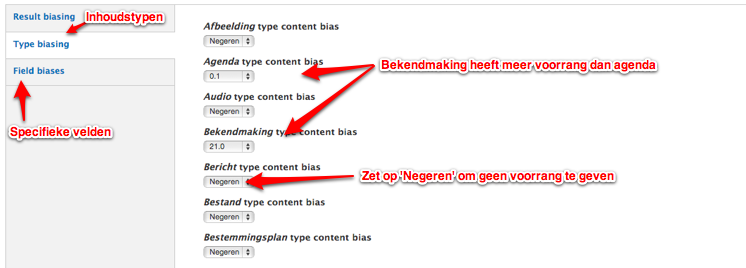
\includegraphics[width=\textwidth]{img/bias.png}
\end{center}

Klik na het bewerken op de knop \emph{Instellingen opslaan} om de \emph{Bias settings} op te slaan. 

\subsubsection{Content uitsluiten van zoekmachine}

Het is mogelijk om specifieke nodes uit te sluiten van indexatie in de interne zoekmachine. Klik onderaan het bewerkformulier op het tabblad \emph{Uitsluiten uit zoekresultaten} en vink de checkbox aan, zie onderataand afbeelding.

\begin{center}
	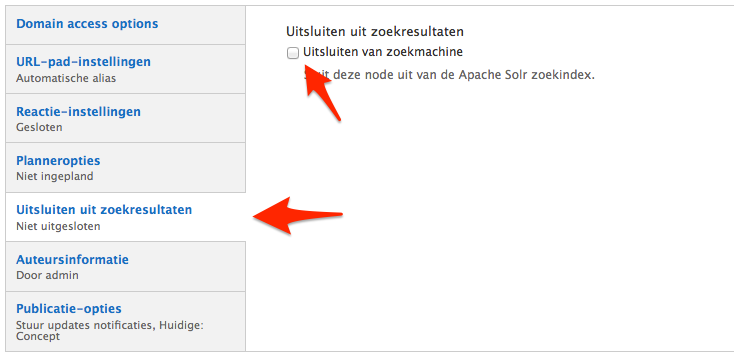
\includegraphics[width=\textwidth]{img/solr-exclude.png}
\end{center}

\subsubsection{Synoniemen beheren}

Solr biedt ondersteuning voor synoniemen. Hiermee kan worden ingesteld dat een zoekopdracht naar "i-pad" ook inhoud met de tekst "ipad" wordt opgenomen in de resultaten.

De synoniemen zijn te beheren via Drupal. Ga hiervoor naar \\ \drupalpath{admin/config/search/apachesolr/synonyms}. Op deze pagina is een lijst te vinden met de huidige synoniemen. Deze kunnen hier worden aangepast of uit de lijst worden gehaald. Onder de lijst is een formulier zichtbaar waarmee nieuwe synoniemen toegevoegd kunnen worden. Het trefwoord is het originele woord (bijv. "ipad") en de synoniemen worden ingevoerd als een komma gescheiden lijst (bijv. "i-pad, i pad").

Nieuwe synoniemen treden niet direct in werking. De lijst wordt iedere nacht doorgezet naar de Solr server. In dit proces wordt tevens de ingestelde lijst samengevoegd met de basislijst (generieke lijst voor alle gemeentes).

\subsection{Afbeeldingsstijlen}\label{afbeeldingsstijlen}

Afbeeldingsstijlen worden gebruikt voor het weergeven van afbeeldingen. Verschillende afbeeldingsstijlen maken het mogelijk een afbeelding op een andere manier (ander formaat bijvoorbeeld) te tonen dan het origineel. 

\subsubsection{Banner}

Banner 

\subsubsection{Full width}

Full width 

\subsubsection{List thumbnail}

List thumbnail 

\subsubsection{Node thumbnail}

Node thumbnail 

\subsubsection{Origineel}

Origineel 

\subsubsection{Overige onderwerp}

Overige onderwerp 

\subsubsection{Portret}

Portret 

\subsubsection{Slide 9/3}

Slide 9/3 

\subsubsection{galleryformatterslide}

galleryformatter slide 

\subsubsection{galleryformatterthumb}

galleryformatter thumb 

\subsubsection{Thumbnail}

thumbnail 

\subsubsection{Medium}

medium 

\subsubsection{Large}

large 

\subsubsection{linkitthumb}

linkut thumb 

\subsubsection{squarethumbnail}

square thumbnail 
\subsection{Abonnementen}\label{abonnementen}
Onderaan detailpagina's van types waarop geabonneerd mag worden staat een formulier om je te abonneren op deze pagina, alle pagina's van dit type of alle pagina's van dit type van deze gebruiker. Selecteer een of meerdere opties en druk op Opslaan.

\begin{center}
	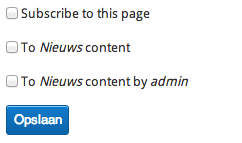
\includegraphics[scale=0.75]{img/abonnementen.png}
\end{center}

Het beheren van de abonnementen staat beschreven in het hoofdstuk \emph{Abonnementen}\seeone{profileabonnementen}.

\subsection{Storingspagina}

Er is een storingspagina aanwezig die getoond wordt bij technische problemen. De tekst van deze pagina is niet redactioneel aan te passen en wordt ingesteld bij installatie.

\subsection{Reageren}

Op de meeste contenttypes kan worden gereageerd. Content types die zijn uitgesloten van reactiemogelijkheden zijn rss, rss\_source (intranet nieuws), slide en editorial (redacitonele blokken).

\subsection{Geocoding}\label{geocoding}

Voor de Google Maps functionaliteit is het mogelijk om automatisch de lengtegraad en breedtegraad op te halen bij de ingevoerde adressen. Hiervoor is een API key noodzakelijk welke aangevraagd kan worden bij Google. De API key kan door een beheerder in Drupal worden ingesteld.
\begin{enumerate}
\item Ga naar \texttt{https://code.google.com/apis/console/} en login met een Google-account
\item Klik in de linkerkolom op \emph{Services}
\item Zet \emph{Google Maps Geolocation API} aan
\item Klik links op \emph{API Access}
\item Kopieer de tekst achter "API key:"
\item Ga naar \texttt{admin/config/content/location/geocoding}
\item Kies voor \emph{Google Maps} bij \emph{Nederland}
\item Sla de settings op
\item Klik op \emph{Parameters instellen} achter \emph{Nederland}
\item Vul de API key in
\item Klik op \emph{Instellingen opslaan}
\end{enumerate}
